%\section{対象計算領域の設定} \label{sec:domain}
\section{\SecBasicDomainSetting} \label{sec:domain}
%=======================================================================

%\Item{\SubsecRelationOfResoGridProcess}
まず、\scalerm での対象計算領域の格子点数とMPIプロセスの関係を整理しておく。
計算領域は、水平格子間隔と格子点数およびMPIプロセス数を指定することで決定されるようになっている。
図\ref{fig:domain}は、
計算領域、水平格子間隔、格子数、及びMPIプロセス数の関係を示している。
水平方向に2次元の領域分割を行うことで並列化がなされている。

格子点数およびMPIプロセス数は、
\namelist{PARAM_INDEX}内の\nmitem{IMAX,JMAX}、\\
\namelist{PARAM_PRC}内の\nmitem{PRC_NUM_X,PRC_NUM_Y}で設定する。
%水平格子間隔については、\namelist{PARAM_GRID}内の\nmitem{DX,DY}で設定する。


図\ref{fig:domain}に示すように、
計算領域全体が、\XDIR に\nmitem{PRC_NUM_X}個、\YDIR に\nmitem{PRC_NUM_Y}個に分割され、それぞれが1つのMPIプロセスによって担当される。

それぞれのMPIプロセスは、\nmitem{IMAX,JMAX,KMAX}個の格子を受け持つ。
ここで、注意すべきことは、「指定する格子点数は各プロセスが受け持つ値」であり、
計算領域全体の格子点数ではないことである。
すなわち、計算領域は、水平格子間隔、格子点数とともにMPIプロセス数にも依存する。


以上の関係から、計算領域全体のそれぞれの方向の格子点数および総格子点数は、
\begin{eqnarray}
&& 領域内{\XDIR} の格子数 = \verb|IMAX| \times \verb|PRC_NUM_X|
   \label{eq:xgridnum}\\
&& 領域内{\YDIR}の格子数 = \verb|JMAX| \times \verb|PRC_NUM_Y|
   \label{eq:ygridnum}\\
&& 領域内の総格子数 = \left(\verb|IMAX| \times \verb|PRC_NUM_X|\right)
   \times (\verb|JMAX| \times \verb|PRC_NUM_Y|)
   \times (\verb|KMAX| )  \nonumber
\end{eqnarray}
となる。
ここで、\nmitem{KMAX}は、鉛直方向の格子点数であり、
\namelist{PARAM_INDEX}内の項目で指定される。

また、領域全体の大きさは、式(\ref{eq:xgridnum}, \ref{eq:ygridnum})を使って、
\begin{eqnarray}
&& {\XDIR}の領域の長さ = {\XDIR}の格子点数 \times \verb|DX| \nonumber\\
&& {\YDIR}の領域の長さ = {\YDIR}の格子点数 \times \verb|DY| \nonumber
\end{eqnarray}
となる。ここで、\nmitem{DX, DY}は、後述するように
\namelist{PRAM_GRID}で指定されるものである。
解像度と領域の大きさが決まっている場合、MPIプロセス数が決まると、
逆算してMPIプロセスあたりの格子点数が決まる。

次節以降では、MPIプロセス数、格子数、格子間隔、
それぞれの設定方法について詳しく説明する。
また、本節内の設定は、
\textcolor{red}{基本的に\texttt{pp.conf}, \texttt{init.conf}, \texttt{run.conf}の設定ファイル間で一致させなければならない}
ことに注意が必要である。


\begin{figure}[h]
\begin{center}
  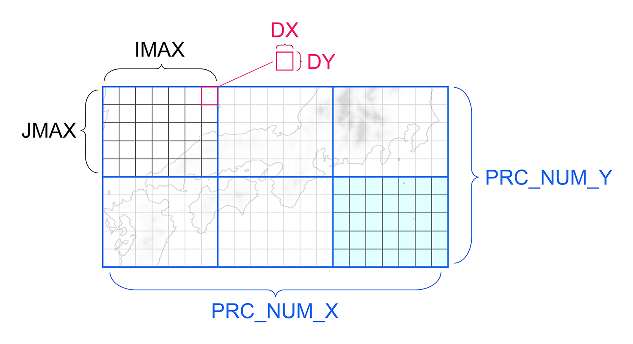
\includegraphics[width=0.8\hsize]{./figure/domain_decomposition.eps}\\
  \caption{計算領域に対する、水平格子間隔(\texttt{DX}, \texttt{DY})、MPIプロセスあたりの格子数(\texttt{IMAX}, \texttt{JMAX})、MPIプロセス数(\texttt{PRC\_NUM\_X}, \texttt{PRC\_NUM\_Y})の関係。水色領域は、ある1つのMPIプロセスが担当する領域。}
  \label{fig:domain}
\end{center}
\end{figure}



\subsection{\SubsecMPIProcess} \label{subsec:relation_dom_reso2}

MPIプロセス数は、設定ファイルの\namelist{PARAM_PRC}で指定する。
\scalerm の入出力ファイルは、MPIプロセス毎に分割されているため、
MPIプロセス数を変更すると分割ファイル数も必ず変わることになる。
従って、例えば、2-MPI並列用に作成した初期値ファイルは、
4-MPI並列のモデル実行には使用できない。
MPIプロセス数を変更するには、
\verb|pp.conf|、\verb|init.conf|、\verb|run.conf| の
すべてを編集・変更し、\verb|pp|、\verb|init| から行う必要がある。\\

\noindent {\small {\gt
\ovalbox{
\begin{tabularx}{140mm}{lX}
\verb|&PARAM_PRC| & \\
\verb| PRC_NUM_X       = 2,| & ; {\XDIR}(東西方向)のMPI並列分割数 \\
\verb| PRC_NUM_Y       = 1,| & ; {\YDIR}(南北方向)のMPI並列分割数 \\
\verb|/|\\
\end{tabularx}
}}}\\


総MPIプロセス数は、\verb|PRC_NUM_X| $\times$ \verb|PRC_NUM_Y|  となり、
上記の例では、\XDIR に2分割、\YDIR に1分割(分割なし)の 2-MPI並列ということになる。

実行時にMPIコマンドに指定するMPIプロセス数は、総MPIプロセス数を指定しなければならない。
この条件を満たさない場合は、下記のメッセージが
標準出力に出力されて計算は行われず、直ちに終了する。

\noindent {\small {\gt
\ovalbox{
\begin{tabularx}{140mm}{l}
\verb|xxx total number of node does not match that requested. Check!| \\
\end{tabularx}
}}}\\





\subsection{\SubsecGridNumSettng} \label{subsec:relation_dom_reso3}
%-----------------------------------------------------------------------

格子数の設定は、設定ファイル(\verb|***.conf|)の\namelist{PARAM_INDEX}で行う。
以下で設定する水平格子数の値は、1つのMPIプロセス当たりの値であることに注意が必要である。\\

\noindent {\small {\gt
\ovalbox{
\begin{tabularx}{140mm}{lX}
\verb|&PARAM_INDEX| & \\
\verb| KMAX = 97,|  & ; 鉛直層数 \\
\verb| IMAX = 20,|  & ; プロセスあたりの{\XDIR}の格子点数 \\
\verb| JMAX = 25,|  & ; プロセスあたりの{\YDIR}の格子点数 \\
\verb|/|\\
\end{tabularx}
}}}\\



\subsection{\SubsecGridIntvSettng} \label{subsec:gridinterv}
%-----------------------------------------------------------------------
\scalerm では、第\ref{subsec:buffer}節で述べる緩和領域を除き、
水平格子間隔は等間隔でのみ設定可能である。
鉛直格子間隔については、任意に定義することが可能である。
すべての方向について等間隔で設定する場合には、以下のように
設定ファイルの\namelist{PARAM_GRID}の\nmitem{DX,DY,DZ}に
それぞれ、東西、南北、鉛直方向の格子間隔を指定する。
単位は[m]である。\\

\noindent {\small {\gt
\ovalbox{
\begin{tabularx}{140mm}{lX}
\verb|&PARAM_GRID  | & \\
\verb| DX = 500.D0,| & ; {\XDIR}(東西方向)の格子間隔\\
\verb| DY = 500.D0,| & ; {\YDIR}(南北方向)の格子間隔\\
\verb| DZ = 500.D0,| & ; {\ZDIR}(鉛直方向)の格子間隔\\
\verb|/|\\
\end{tabularx}
}}}\\


以下に、鉛直方向での任意の格子点位置を指定する場合の設定を示す。
鉛直方向は、ローレンツ格子を採用しており、
速度成分定義格子点とスカラー定義格子点が半格子分ずれた食い違い格子になっている。
ここでは、スカラー量を定義している格子点をセンターポイントと呼び、
半格子ズレた格子点をフェイスポイントと呼ぶ。

直接格子点の位置を指定する場合は、フェイスポイントの位置を
\namelist{PARAM_GRID}の中の\nmitem{FZ(:)}で配列として与えればよい
\footnote{指定の際には、シミュレーションの計算精度
(モデルのコンパイル時に指定した浮動小数点の精度。デフォルトでは倍精度)を用いることが望ましい。}
(図\ref{fig:scale_grid}参照)。
また、\nmitem{FZ(:)}で指定する値の数は、鉛直層数
(\namelist{PARAM_INDEX}の\nmitem{KMAX})と一致している必要がある。
例として理想実験のチュートリアルの設定ファイルの例を下記に示す。\\

\noindent {\small {\gt
\ovalbox{
\begin{tabularx}{140mm}{lX}
\verb|&PARAM_GRID|     & \\
\verb| DX = 500.D0,|   & {\XDIR} の格子間隔(等間隔)[m]\\
\verb| DY = 500.D0,|   & {\YDIR}の格子間隔(等間隔)[m]\\
\verb| FZ(:) = |       & {\ZDIR}のフェイスポイントの位置[m] \\
\verb|    80.000000000000000      ,| & \\
\verb|    168.00000190734863      ,| & \\
\verb|    264.80000610351567      ,| & \\
\verb|     〜 中略 〜|           & \\
\verb|    14910.428862936289      ,| & \\
\verb|    15517.262523292475      ,| & \\
\verb|    16215.121232702089      ,| & \\
\verb|    17017.658748523147      ,| & \\
\verb|    17940.576891717363      ,| & \\
\verb|    19001.932756390710      ,| & \\
\verb|    20222.492000765058      ,| & \\
\verb| BUFFER_DZ = 5000.D0,|          & 第\ref{subsec:buffer}節参照\\
\verb| BUFFFACT  =   1.0D0,|          & 第\ref{subsec:buffer}節参照\\
\verb|/|\\
\end{tabularx}
}}}\\


\begin{figure}[tb]
\begin{center}
  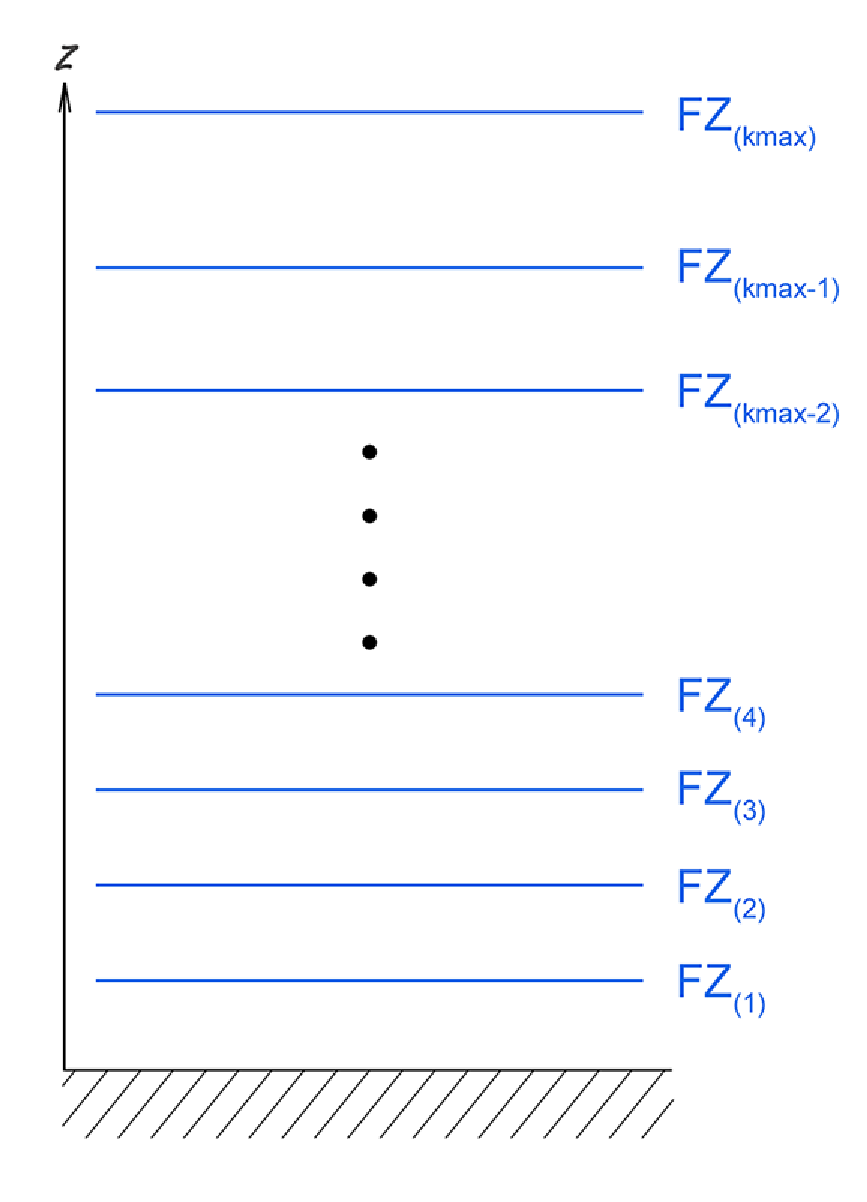
\includegraphics[width=0.4\hsize]{./figure/verticalface.eps}\\
  \caption{\scalerm の鉛直格子のフェイスポイントの定義点。\namelist{PARAM_GRID}で\nmitem{FZ}を指定する時は、地表面を除いた計算領域下端第1層目上端の位置から$k=1$として与える。}
  \label{fig:scale_grid}
\end{center}
\end{figure}

なお、指定された鉛直高度は
標高が0 mの場所(海上)での鉛直格子点位置として設定され、標高がある場所では地形に沿った座標系によって適切に処理される。


格子点位置は任意に設定できるが、設定によっては計算不安定につながる。
鉛直層の設定については、作成をサポートするツールが、\texttt{scale-\version/scale-rm/util/makevgrid/}
ディレクトリの中に \verb|make_vgrid.f90|というFortranプログラムと
いくつかのサンプルネームリストが用意されているので、参考にされたい。
ツールをコンパイルして実行すれば直ちに設定ファイルに貼り付けて使用できる
\nmitem{FZ(:)}の値が作成される。


\subsection{\SecBasicBufferSetting} \label{subsec:buffer}
%-----------------------------------------------------------------------
モデル最上層では音波や重力波の非物理的な反射が起こる。
また、側面境界では現実大気実験を行う際に境界条件として与えられる入力データと
対象領域の計算結果の間に値の不一致が起こる。
これを回避するため、「緩和領域」を設ける。

\scalerm では計算領域の境界のすぐ内側に緩和領域を設定することができる
(図\ref{fig:buff_xz})。
緩和領域の格子では、計算された値を
指定された値(境界値データ、親領域のデータなど)に対して
ある時定数で近づける。以下これをナッジングと呼ぶ(上層における緩和はレイリーダンピングと呼ばれることが多い)。
緩和領域の幅は、設定ファイルの\namelist{PARAM_GRID}の中で設定する。
以下に例を示す。
設定はすべての設定ファイルにおいて共通していなければならない。\\

~\\
\proofcomment{(八代)「条件と領域の間」という言葉の使い方が直感的にわかりません。} \\
\replycomment{(足立) なおしましたー} \\
~\\

\noindent {\small {\gt
\ovalbox{
\begin{tabularx}{150mm}{lX}
\verb|&PARAM_GRID  |            & \\
 \verb|BUFFER_DZ = 5000.D0,   | & ; {\ZDIR}(モデルトップから下向き方向)の緩和領域の幅(参考値) [m]\\
 \verb|BUFFER_DX = 300000.D0, | & ; {\XDIR}(東西方向)の緩和領域の幅(参考値) [m]\\
 \verb|BUFFER_DY = 300000.D0, | & ; {\YDIR}(南北方向)の緩和領域の幅(参考値) [m]\\
 \verb|BUFFFACT  = 1.D0,      | & ; 緩和領域内の格子間隔に対するストレッチ係数(デフォルトは1.0)\\
\verb|/|\\
\end{tabularx}
}}}\\


%
水平方向には東西南北の四方境界に緩和領域が設定されるが、
鉛直方向には計算領域の上端にのみ緩和領域が設定され、下端には設定されない。
緩和領域は、計算領域内に設定されるため、
ナッジングの影響を受けない領域(緩和領域を除いた範囲)は
計算領域よりも狭くなることに注意が必要である。

緩和領域の格子数 \verb|ibuff|は、
\[
\sum_{n=1}^{\verb|ibuff|} \verb|BDX|(n) \ge \nmitemeq{BUFFER_DX} \nonumber
\]
の関係を満たす最小の整数で自動的に計算される。
したがって、緩和領域の大きさ $\verb|BUFFER|_{\verb|X|}$ ($= \sum_{n=1}^{\verb|ibuff|} \verb|BDX|(n)$)
は必ずしも \nmitem{BUFFER_DX} と一致するわけではないことに注意が必要である。
結局、緩和領域を除いた計算領域の大きさは、
\[
\nmitemeq{DX} \times ( \nmitemeq{IMAX} \times \nmitemeq{PRC_NUM_X} - 2 \times \verb|ibuff| )
\]
となる。

ここでは、{\XDIR}の説明をしたが、{\YDIR}、{\ZDIR}も同様である。
ただし、{\ZDIR} については下端には緩和領域が取られないため、緩和領域を除いた計算領域の大きさは、モデル上端の緩和領域の格子数を\verb|kbuff|として
\[
\nmitemeq{DZ} \times ( \nmitemeq{KMAX} - \verb|kbuff| )
\]
となる。


\begin{figure}[t]
\begin{center}
  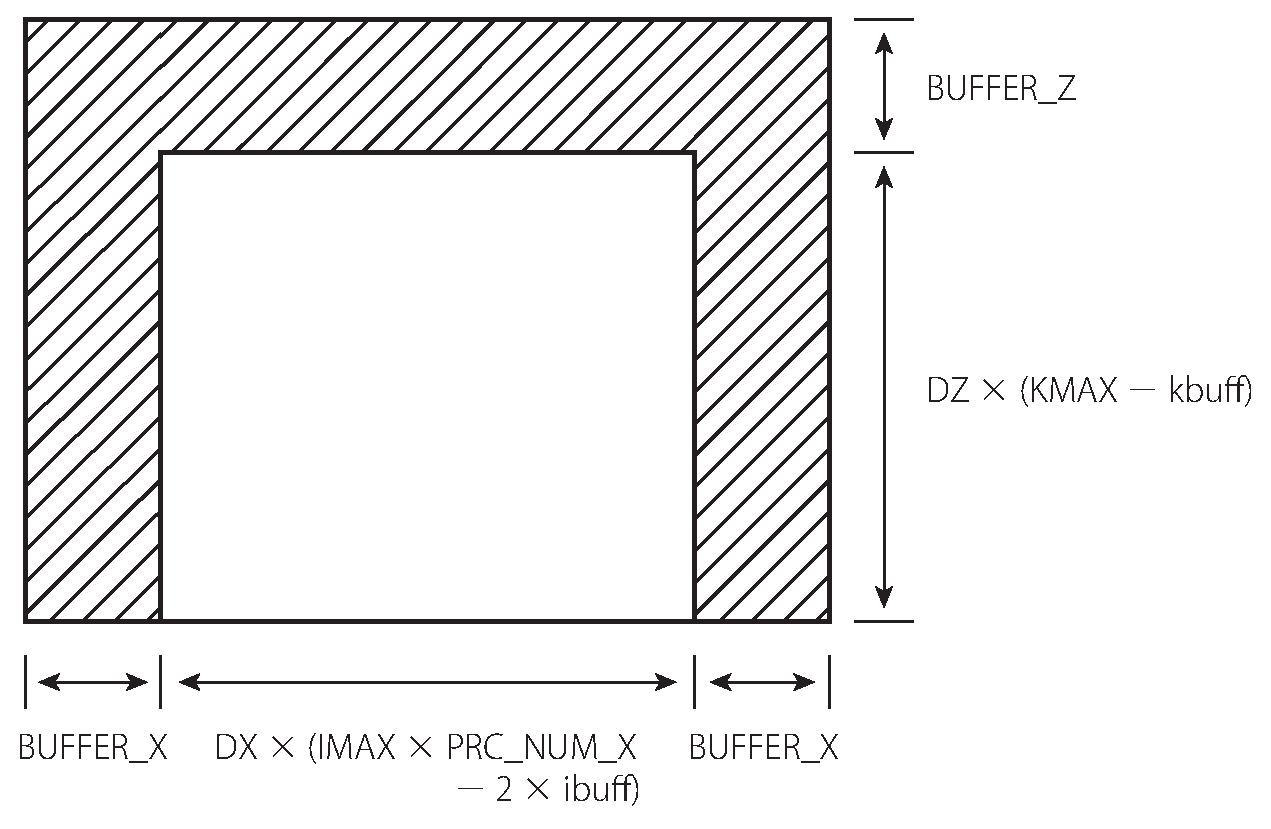
\includegraphics[width=0.8\hsize]{./figure/buffer_xz.eps}\\
  \caption{計算領域における緩和領域の配置:斜線部分が緩和領域を意味する。
  図はXZ断面だが、Y方向にも同一の配置である。}
  \label{fig:buff_xz}
\end{center}
\end{figure}


一般に、緩和領域の大きさや緩和格子点の数のとり方については、
解く問題に依存するため明確な指標はない。
\scalerm では、鉛直方向(計算領域トップ)の緩和格子点は5点以上、
水平方向(側面境界付近)の緩和格子点は20〜40点程度を推奨している。
実験設定や事例によっては、さらに緩和格子点を増やしたり、
後述のストレッチ係数を用いて緩和領域を広げたり、
緩和の時定数を調整したりする必要があるだろう。
時定数とは、目標値との差が$1/e$になるまでの時間である。
緩和の時定数は、
\namelist{PARAM_ATMOS_BOUNDARY}の中の
\nmitem{ATMOS_BOUNDARY_taux, ATMOS_BOUNDARY_tauy, ATMOS_BOUNDARY_tauz}によって秒単位で設定する。
デフォルトの値は $10 \Delta t$ であり、これは、10タイムステップで$1/e$になることに相当する。
タイムステップについては、第\ref{sec:timeintiv}節を参照のこと。

\subsubsection{緩和領域の格子間隔をストレッチさせる}

緩和領域の格子間隔は、基本的に
\namelist{PARAM_GRID}の中の\nmitem{DX, DY, DZ}で指定した通りであるが、
\nmitem{BUFFFACT}に1以上の値を設定することで、ストレッチさせることも可能である。
ただし、格子間隔を等間隔で指定した場合、
この\nmitem{BUFFFACT}の設定は、X、Y、{\ZDIR}すべてに適用される。
それぞれの方向に別々に設定したい場合は、\nmitem{BUFFFACT_X, BUFFFACT_Y, BUFFFACT_Z}を指定する。
{\ZDIR}の層レベルを任意の格子点位置に指定する場合、
すなわち、\nmitem{FZ(:)}を与える場合(第\ref{subsec:gridinterv}節参照のこと)にはストレッチの設定は{\ZDIR}には適用されない。

緩和領域内の格子間隔 (\verb|BDX|) は次の通り決定される。
\begin{eqnarray}
 \verb|BDX(|n\verb|)| &=& \verb|DX| \times \verb|BUFFFACT|^n \nonumber
\end{eqnarray}
ここで、$n$は緩和領域内の格子点番号を表し、計算領域の内側から外側へ向う番号である。
緩和領域の格子間隔は、
\nmitem{BUFFFACT=1.0}ならば内部領域と同じであり、
\nmitem{BUFFFACT=1.2}ならば内側から外側(境界)に向かって1.2倍の割合で広がっていく。
\nmitem{BUFFFACT}はいくつに設定しても良いが、計算の安定性を考慮すると 1.0から1.2 が推奨される。


緩和領域の大きさ$\verb|BUFFER|_{\verb|X|}$は、
\[
  \verb|BUFFER|_{\verb|X|} = \nmitemeq{DX} \times \frac{ \nmitemeq{BUFFFACT}^{\texttt{\detokenize{ibuff}}}-1}{ \nmitemeq{BUFFFACT}-1 }
\]
となる。
%
緩和領域の幅\nmitem{BUFFER_DX}が同じでも、
\nmitem{BUFFFACT}の値を大きくすると緩和領域の格子数は少なくなる。

